\documentclass[aspectratio=169, 10pt]{beamer}

% Typography and encoding
\usepackage[utf8]{inputenc}
\usepackage[T1]{fontenc}
\usepackage{helvet}
\usepackage{microtype}
\usepackage{amsmath, amssymb, amsfonts}
\usepackage{booktabs}
\usepackage{graphicx}
\usepackage{xcolor}
\usepackage{colortbl}

% Define modern academic theme colors
\definecolor{primary}{RGB}{30, 41, 59}     % Slate dark
\definecolor{accent}{RGB}{15, 118, 110}    % Teal
\definecolor{highlight}{RGB}{185, 28, 28}  % Crimson
\definecolor{subtle}{RGB}{100, 116, 139}   % Muted gray
\definecolor{cardbg}{RGB}{248, 250, 252}   % Off-white

\setbeamercolor{palette primary}{bg=primary, fg=white}
\setbeamercolor{structure}{fg=accent}
\setbeamercolor{title}{fg=white, bg=primary}
\setbeamercolor{frametitle}{fg=primary, bg=cardbg}
\setbeamercolor{block title}{fg=white, bg=accent}
\setbeamercolor{block body}{fg=primary, bg=cardbg}

\setbeamertemplate{navigation symbols}{}
\setbeamertemplate{footline}{
    \leavevmode%
    \hbox{%
        \begin{beamercolorbox}[wd=\paperwidth,ht=2.2ex,dp=0.8ex,leftskip=0.8cm,rightskip=0.8cm]{cardbg}%
            \tiny\textcolor{subtle}{NLP1 (MSc AI) \textbar{} Project 1: TweetEval Sentiment Classification \hfill Slide \insertframenumber{} / 6}
        \end{beamercolorbox}%
    }%
    \vskip0pt%
}

\setbeamertemplate{frametitle}{
    \begin{beamercolorbox}[wd=\paperwidth,ht=2.4ex,dp=0.7ex,leftskip=0.6cm]{frametitle}
        \textbf{\normalsize\insertframetitle} \hfill \scriptsize\textcolor{accent}{\insertframesubtitle}\hspace*{0.6cm}
    \end{beamercolorbox}
}

\begin{document}

% ==============================================================================
% SLIDE 1: DATASET CHOICE & EXPLORATORY DATA ANALYSIS (EDA)
% ==============================================================================
\begin{frame}[shrink=8]{1. Dataset \& Exploratory Data Analysis (EDA)}{Topic 1: Split Sizes, Temporal Prior Shift \& Evaluation Metric}
\begin{columns}[T]
\begin{column}{0.53\textwidth}
    \scriptsize
    \textbf{Task \& Dataset Selection}:
    \begin{itemize}\setlength\itemsep{1.5pt}
        \item \textbf{Benchmark}: \texttt{cardiffnlp/tweet\_eval} (3-class Sentiment: Neg, Neu, Pos).
        \item \textbf{Split Sizes}: $45,615$ Train $\mid$ $2,000$ Validation $\mid$ $12,284$ Official Test.
    \end{itemize}
    \vspace{2pt}
    \textbf{Critical Finding: Severe Temporal Prior Shift}:
    \begin{itemize}\setlength\itemsep{1.5pt}
        \item \textbf{Train / Val}: $15.5\%$ Negative, $45.3\%$ Neutral, $39.1\%$ Positive.
        \item \textbf{Official Test}: \textbf{32.3\% Negative} ($\mathbf{\times 2.1}$ doubles!), $48.3\%$ Neutral, \textbf{19.3\% Positive} ($\mathbf{\times 0.5}$ halves!).
        \item \emph{Why Macro-F1}: Raw accuracy is misleading under prior shift. \textbf{Macro-F1} ($\frac{1}{3}\sum_{c} F_{1,c}$) weights all three classes equally.
        \item \emph{Class-Weighted Loss}: Inverse frequency weights $w_c \propto 1/N_c$ prevent the majority Neutral class from overwhelming minority Negative gradients.
    \end{itemize}
    \vspace{2pt}
    \textbf{Twitter Stylometrics}:
    \begin{itemize}\setlength\itemsep{1.5pt}
        \item Mean length: $19.4$ words/tweet; noisy syntax, user mentions, hashtags, slang.
        \item \textbf{Negations}: $3\times$ more frequent in Negative ($0.224$) vs. Positive ($0.079$).
        \item \textbf{Exclamations}: $3\times$ more frequent in Positive ($0.468$) vs. Negative ($0.157$).
    \end{itemize}
\end{column}
\begin{column}{0.45\textwidth}
    \centering
    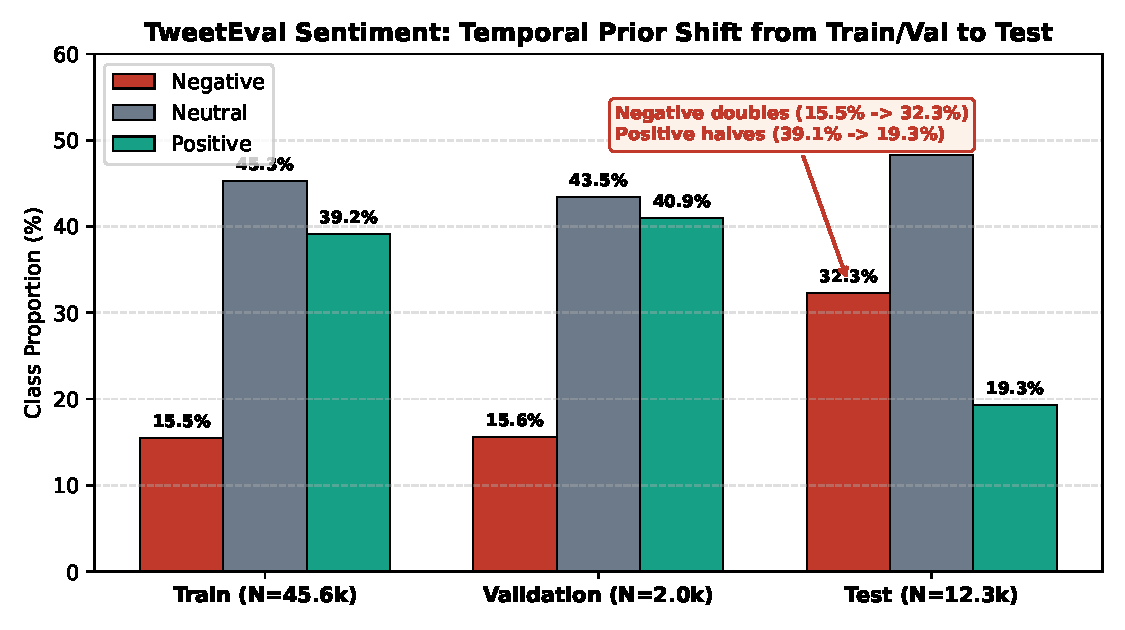
\includegraphics[width=\linewidth, height=0.72\textheight, keepaspectratio]{figures/minimal_class_distribution.pdf}
    \vspace{2pt}
    \begin{block}{Dataset \& Metric Summary}
        \scriptsize Because Negative tweets double in the test set ($15.5\% \to 32.3\%$), Macro-F1 and class weighting are essential for fair evaluation.
    \end{block}
\end{column}
\end{columns}
\end{frame}

% ==============================================================================
% SLIDE 2: TEXT SEGMENTATION & TOKENIZER DESIGN
% ==============================================================================
\begin{frame}[shrink=8]{2. Text Segmentation: Comparing 3 Tokenizers}{Topic 2: Whitespace vs. NLTK TweetTokenizer vs. Subword BPE}
\begin{columns}[T]
\begin{column}{0.53\textwidth}
    \scriptsize
    \textbf{Comparing Three Tokenization Strategies}:
    \begin{enumerate}\setlength\itemsep{1.5pt}
        \item \textbf{Whitespace (\texttt{text.split()})}: $V=43,395$, $19.44$ toks/tweet (ratio $1.00$). Leaves punctuation glued to words (\texttt{"it..."}); high OOV rate on unseen tweets.
        \item \textbf{NLTK \texttt{TweetTokenizer} (Social Regex)}: $V=43,395$, $22.81$ toks/tweet (ratio $1.17$). Preserves emoticons (\texttt{:-)}), strips \texttt{@handles}, normalizes repeated chars (\texttt{cooool} $\to$ \texttt{coool}). Moderate OOV on novel typos/slang.
        \item \textbf{Subword Byte-Level BPE}: Trained in-domain on training tweets $\Rightarrow$ \textbf{0.00\% UNK rate}. Splits rare words into reusable subword stems and affixes.
    \end{enumerate}
    \vspace{2pt}
    \textbf{Byte-BPE Vocabulary Sweep ($V \in \{2\text{k}, 4\text{k}, 8\text{k}, 16\text{k}\}$)}:
    \begin{itemize}\setlength\itemsep{1.2pt}
        \item $V=2,048$: Over-fragmented into short pieces ($37.28$ toks/tweet, $1.92$ ratio).
        \item $\mathbf{V=8,192}$ \textbf{(Selected)}: $29.64$ toks/tweet ($1.52$ ratio). Sweet spot: preserves stems while keeping sentiment affixes (\texttt{un-}, \texttt{dis-}, \texttt{'t}) with $0\%$ UNK.
        \item $V=16,384$: $27.55$ toks/tweet ($1.42$ ratio); memorizes rare noise, doubles params.
    \end{itemize}
    \vspace{1pt}
    \tiny\texttt{Ex: "cooool :-) didn't"} $\to$ \textbf{TweetTok}: \texttt{['coool', ':-)', "didn't"]} $\mid$ \textbf{BPE-8k}: \texttt{['c', 'oo', 'ool', 'Ġ:-)', 'Ġdidn', "'t"]}
\end{column}
\begin{column}{0.45\textwidth}
    \centering
    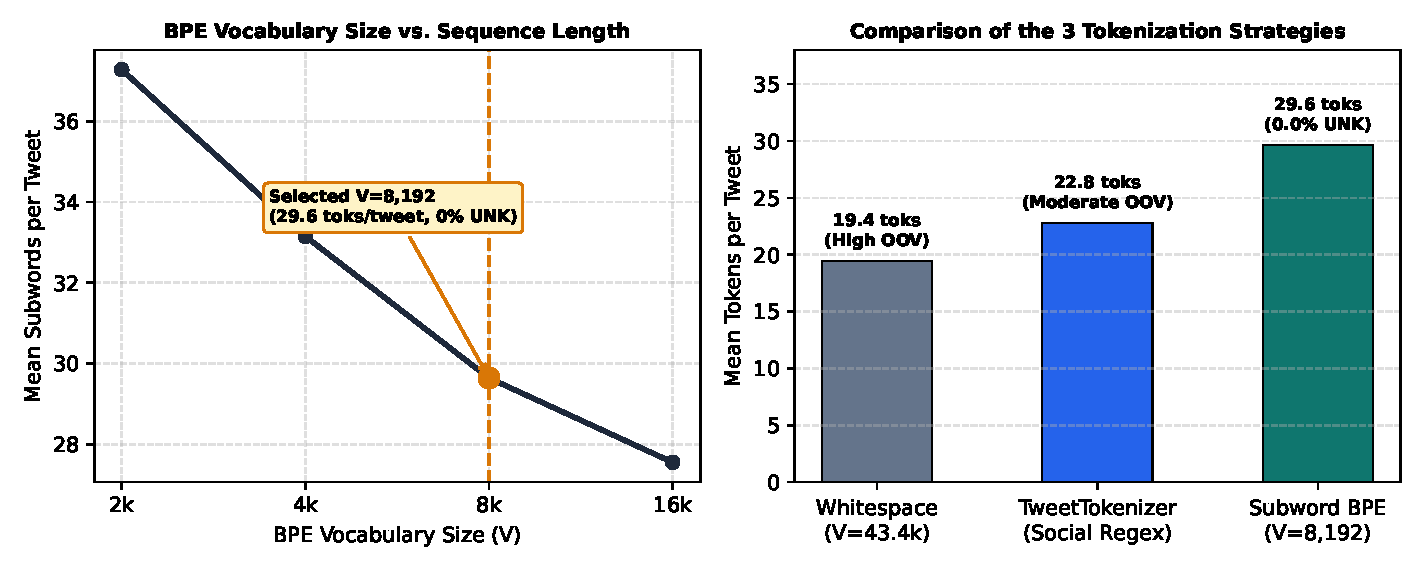
\includegraphics[width=\linewidth, height=0.72\textheight, keepaspectratio]{figures/minimal_vocab_sweep.pdf}
    \vspace{2pt}
    \begin{block}{Segmentation Takeaway}
        \scriptsize Rule-based \texttt{TweetTokenizer} normalizes social media syntax for word embeddings, while BPE ($V=8,192$) ensures $0.00\%$ OOV and morphological sharing.
    \end{block}
\end{column}
\end{columns}
\end{frame}

% ==============================================================================
% SLIDE 3: REPRESENTATION SPACES (FEATURE ENGINEERING)
% ==============================================================================
\begin{frame}[shrink=8]{3. Document Representations: Sparse vs. Pre-Trained Dense}{Topic 3: Sparse Subwords vs. Pre-Trained GloVe Twitter Embeddings}
\begin{columns}[T]
\begin{column}{0.53\textwidth}
    \scriptsize
    \textbf{Three Sparse Subword Spaces (BPE, $V = 8,192$, $99.71\%$ Zeros)}:
    \begin{enumerate}\setlength\itemsep{1.2pt}
        \item \textbf{Binary Token Indicator}: $x_i \in \{0, 1\}$. Marks presence/absence. Since subwords repeat in $<2.4\%$ of tweet positions, indicator captures $\sim 97.6\%$ of count information.
        \item \textbf{Bag-of-Words (BoW) Counts}: $x_i = \text{count}(i, d) \in \mathbb{N}_0$. Preserves raw count magnitude for repeated punctuation (\texttt{!!!}) and intensifiers.
        \item \textbf{Subword TF-IDF}: $x_i = \text{TF}(i, d) \cdot \text{IDF}(i)$ with $L_2$ normalization ($\|x\|_2=1$). On short tweets, $L_2$ normalization penalizes tweets with neutral filler words by shrinking the magnitude of strong sentiment tokens.
    \end{enumerate}
    \vspace{2pt}
    \textbf{Pre-Trained Dense Twitter Embeddings (\texttt{glove-twitter-25}, $D = 25$)}:
    \begin{itemize}\setlength\itemsep{1.2pt}
        \item Pre-trained on 2B tweets ($1.19\text{M}$ word vocabulary, $0\%$ zeros).
        \item Captures continuous synonymy (\texttt{cos(good, great)=0.94}, \texttt{cos(love, like)=0.90}), whereas sparse BoW treats all distinct words as orthogonal ($\cos = 0$).
        \item \textbf{Mean-Pooled ($\mathbb{R}^{25}$)}: Orderless average vector (for Log-Linear \& Shallow MLP).
        \item \textbf{Sequential ($\mathbb{R}^{T \times 25}$)}: Preserves ordered trajectory $[e(w_1), \dots, e(w_T)]$ (for BiLSTM).
    \end{itemize}
\end{column}
\begin{column}{0.45\textwidth}
    \centering
    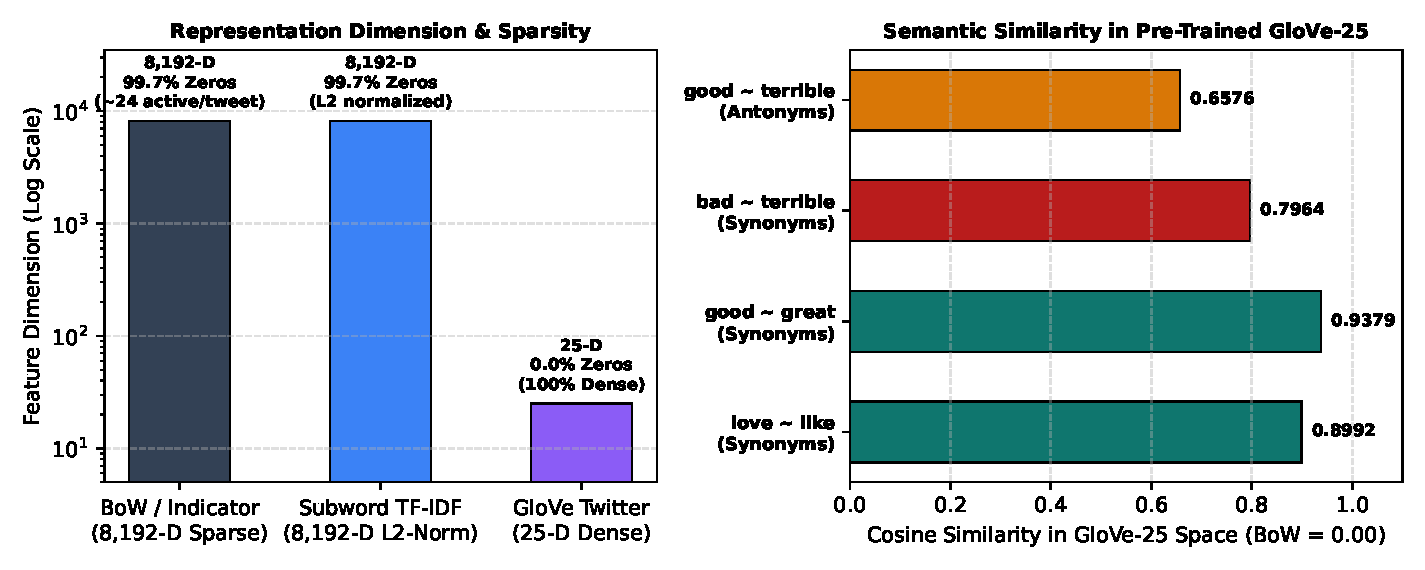
\includegraphics[width=\linewidth, height=0.72\textheight, keepaspectratio]{figures/minimal_representations_polarity.pdf}
    \vspace{2pt}
    \begin{block}{Interpretability of Semantic Clustering}
        \scriptsize Cosine similarities in GloVe: \texttt{good} $\approx$ \texttt{great} ($0.94$), \texttt{love} $\approx$ \texttt{like} ($0.90$), \texttt{bad} $\approx$ \texttt{terrible} ($0.80$). Dense embeddings group synonyms into semantic neighborhoods.
    \end{block}
\end{column}
\end{columns}
\end{frame}

% ==============================================================================
% SLIDE 4: MODEL ARCHITECTURES & FAIR HYPOTHESES
% ==============================================================================
\begin{frame}[shrink=8]{4. Model Architectures \& Fair Hypotheses}{Topic 4: Log-Linear, Shallow MLP \& Bidirectional LSTM}
\begin{columns}[T]
\begin{column}{0.53\textwidth}
    \scriptsize
    \textbf{Three Clean Architectures Evaluated}:
    \begin{enumerate}\setlength\itemsep{1.2pt}
        \item \textbf{Log-Linear Softmax}: $\hat{y} = \text{softmax}(W x + b)$. Direct linear decision boundary ($24,579$ params on BoW; only $78$ params on 25-D GloVe).
        \item \textbf{Shallow MLP}: $\text{Linear}(D, 256) \to \text{ReLU} \to \text{Dropout}(0.25) \to \text{Linear}(256, 3)$. Single hidden layer with non-linear activation ($2.10\text{M}$ params on BoW; $7,427$ on GloVe).
        \item \textbf{Bidirectional LSTM}: $\text{BiLSTM}(25, 64) \to \text{MeanPool} \to \text{Linear}(128, 3)$. Sequential recurrence ($96,643$ parameters).
    \end{enumerate}
    \vspace{2pt}
    \textbf{Three Fair Experimental Hypotheses}:
    \begin{itemize}\setlength\itemsep{1.2pt}
        \item \textbf{H1 (Sparse BoW, 8,192-D)}: Log-Linear ($24,579$ params) vs. Shallow MLP ($2,098,051$ params). High-dimensional BoW is already linearly separable $\Rightarrow$ MLP adds no gain.
        \item \textbf{H2 (Dense GloVe-25 Mean-Pool)}: Log-Linear ($78$ params) vs. Shallow MLP ($7,427$ params). A flat plane underfits 25-D space $\Rightarrow$ non-linear ReLU yields $+11.5\%$ F1.
        \item \textbf{H3 (Fair MLP vs. LSTM on Dense GloVe-25)}: Shallow MLP (Mean-Pooled $\mathbb{R}^{25}$) vs. BiLSTM (Sequential $\mathbb{R}^{T \times 25}$). Exact same \texttt{TweetTokenizer} + \texttt{glove-twitter-25} embeddings $\Rightarrow$ sequential recurrence captures word order \& negation!
    \end{itemize}
\end{column}
\begin{column}{0.45\textwidth}
    \centering
    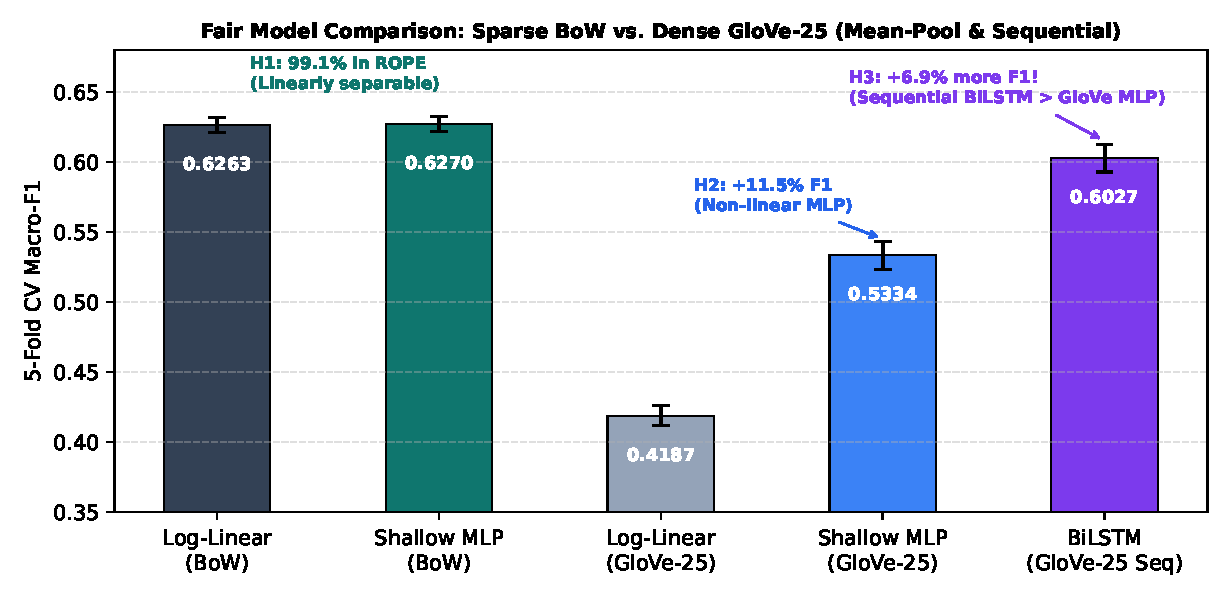
\includegraphics[width=\linewidth, height=0.48\textheight, keepaspectratio]{figures/minimal_architectures_ablation.pdf}
    \vspace{2pt}
    \begin{block}{Architecture Complexity Matrix}
    \centering
    \scriptsize
    \resizebox{\linewidth}{!}{%
    \begin{tabular}{l@{\hspace{4pt}}l@{\hspace{4pt}}r@{\hspace{4pt}}l}
        \toprule
        \textbf{Model Architecture} & \textbf{Input Space} & \textbf{Params} & \textbf{Hypothesis Tested} \\
        \midrule
        Log-Linear & Sparse BoW ($8,192$-D) & 24,579 & H1 Baseline (Linear) \\
        Shallow MLP & Sparse BoW ($8,192$-D) & 2,098,051 & H1 Test (Non-linear) \\
        Log-Linear & GloVe Mean-Pool ($25$-D) & 78 & H2 Baseline (Flat plane) \\
        Shallow MLP & GloVe Mean-Pool ($25$-D) & 7,427 & H2 Test / H3 Baseline \\
        Bidirectional LSTM & GloVe Sequence ($T \times 25$) & 96,643 & H3 Fair Sequential Test \\
        \bottomrule
    \end{tabular}%
    }
    \end{block}
\end{column}
\end{columns}
\end{frame}

% ==============================================================================
% SLIDE 5: 5-FOLD STRATIFIED CV & CORRELATED BAYESIAN ROPE
% ==============================================================================
\begin{frame}[shrink=8]{5. 5-Fold Stratified CV \& Correlated Bayesian ROPE}{Topic 5: Cross-Validation Benchmark \& Statistical ROPE Decisions}
\begin{columns}[T]
\begin{column}{0.54\textwidth}
    \scriptsize
    \textbf{Protocol: 5-Fold Stratified CV ($N=45,615$) \& Bayesian $t$-Test}:
    \begin{itemize}\setlength\itemsep{1pt}
        \item Folds share $80\%$ training data. We use the \textbf{Correlated Bayesian $t$-test} ($\rho = 0.20$) with $\text{ROPE} = [-0.01, +0.01]$ ($\pm 1\%$ Macro-F1).
    \end{itemize}
    \vspace{1pt}
    \resizebox{\linewidth}{!}{%
    \begin{tabular}{l@{\hspace{4pt}}l@{\hspace{4pt}}c@{\hspace{4pt}}c}
        \toprule
        \textbf{Model Configuration} & \textbf{Representation} & \textbf{5-Fold CV Macro-F1} & \textbf{CV Accuracy} \\
        \midrule
        Log-Linear (Indicator) & Binary Indicator ($8,192$-D) & $0.6259 \pm 0.0038$ & $65.10\% \pm 0.43\%$ \\
        \textbf{Log-Linear (BoW)} & \textbf{Bag-of-Words ($8,192$-D)} & $\mathbf{0.6263 \pm 0.0055}$ & $\mathbf{65.08\% \pm 0.56\%}$ \\
        Log-Linear (TF-IDF) & Subword TF-IDF ($8,192$-D) & $0.6058 \pm 0.0028$ & $62.89\% \pm 0.35\%$ \\
        \textbf{Shallow MLP (BoW)} & \textbf{Bag-of-Words ($8,192$-D)} & $\mathbf{0.6270 \pm 0.0054}$ & $\mathbf{65.13\% \pm 0.68\%}$ \\
        Log-Linear (GloVe-25) & GloVe Mean-Pool ($25$-D) & $0.4187 \pm 0.0072$ & $52.84\% \pm 0.81\%$ \\
        Shallow MLP (GloVe-25) & GloVe Mean-Pool ($25$-D) & $0.5334 \pm 0.0100$ & $58.74\% \pm 0.94\%$ \\
        \textbf{BiLSTM (GloVe-25)} & \textbf{GloVe Sequence ($T \times 25$)} & $\mathbf{0.6027 \pm 0.0098}$ & $\mathbf{64.70\% \pm 0.99\%}$ \\
        \bottomrule
    \end{tabular}%
    }
    \vspace{2pt}
    \scriptsize
    \textbf{5 Fair Pairwise Correlated Bayesian Decisions}:
    \begin{itemize}\setlength\itemsep{1pt}
        \item \textbf{BoW vs. Indicator}: $\Delta = +0.0004 \Rightarrow \mathbf{P(\text{ROPE}) = 98.8\%}$ (Equivalence: words rarely repeat).
        \item \textbf{BoW vs. TF-IDF}: $\Delta = +0.0205 \Rightarrow \mathbf{P(\text{BoW} > \text{TF-IDF}) = 99.4\%}$ (BoW wins: $L_2$ norm dilutes).
        \item \textbf{H1 (MLP vs. Log-Lin on BoW)}: $\Delta = +0.0007 \Rightarrow \mathbf{P(\text{ROPE}) = 99.1\%}$ (Practically equivalent!).
        \item \textbf{H2 (MLP vs. Log-Lin on GloVe)}: $\Delta = +0.1147 \Rightarrow \mathbf{P(\text{MLP} > \text{Linear}) = 100\%}$ ($+11.5\%$ F1 jump).
        \item \textbf{H3 (BiLSTM vs. MLP on GloVe)}: $\Delta = +0.0693 \Rightarrow \mathbf{P(\text{LSTM} > \text{MLP}) = 100\%}$ ($+6.9\%$ F1 from sequence!).
    \end{itemize}
\end{column}
\begin{column}{0.44\textwidth}
    \centering
    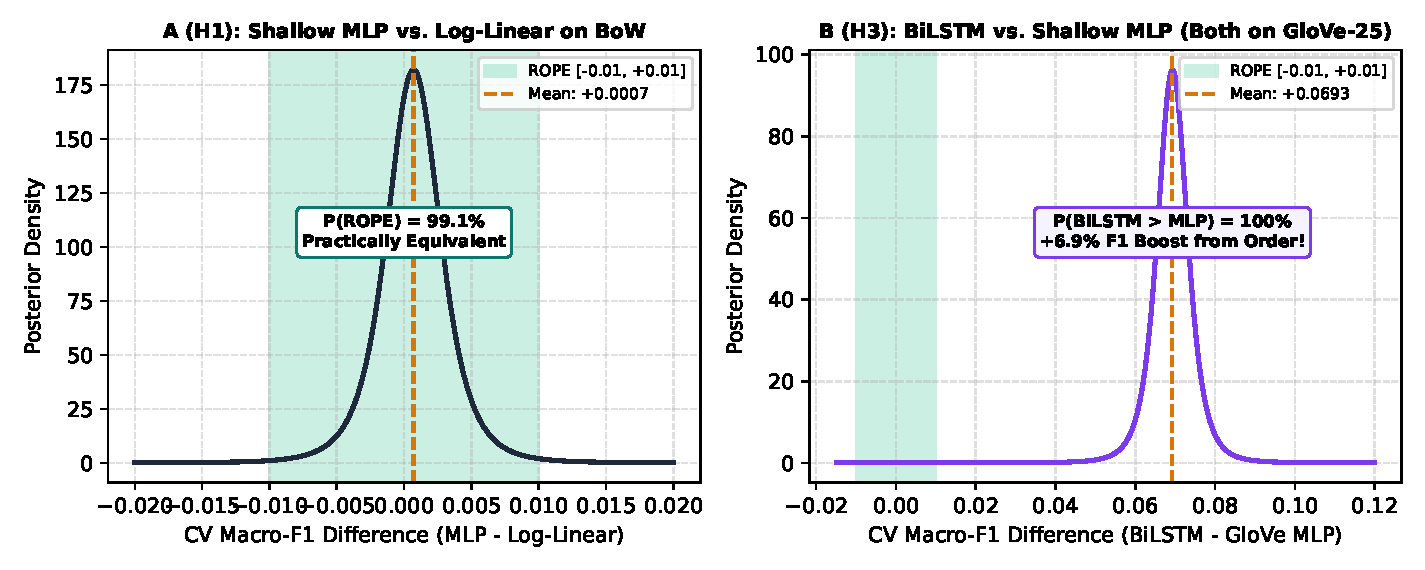
\includegraphics[width=\linewidth, height=0.72\textheight, keepaspectratio]{figures/minimal_bayesian_rope.pdf}
    \vspace{2pt}
    \begin{block}{Statistical Verification Summary}
        \scriptsize ROPE confirms Shallow MLP $\approx$ Log-Linear on BoW ($99.1\%$), while BiLSTM decisively outperforms Shallow MLP on the same GloVe embeddings ($100\%$).
    \end{block}
\end{column}
\end{columns}
\end{frame}

% ==============================================================================
% SLIDE 6: OFFICIAL TEST GENERALIZATION & ERROR ANALYSIS
% ==============================================================================
\begin{frame}[shrink=8]{6. Official Test Set ($N=12,284$) \& Error Analysis}{Topic 6: Test Benchmark, Confusion Matrices \& Failure Modes}
\begin{columns}[T]
\begin{column}{0.54\textwidth}
    \scriptsize
    \textbf{Official Held-Out Test Set Benchmark ($N=12,284$)}:
    \vspace{1pt}
    \resizebox{\linewidth}{!}{%
    \begin{tabular}{l@{\hspace{4pt}}r@{\hspace{4pt}}c@{\hspace{4pt}}c@{\hspace{4pt}}l}
        \toprule
        \textbf{System} & \textbf{Params} & \textbf{Test Macro-F1} & \textbf{Test Acc} & \textbf{Key Characteristic} \\
        \midrule
        \textbf{Log-Linear (BoW)} & \textbf{24,579} & $\mathbf{0.5799}$ & $\mathbf{58.91\%}$ & Selected linear champion (from-scratch) \\
        Shallow MLP (BoW) & 2,098,051 & $0.5862$ & $59.46\%$ & Confirms sparse linear equivalence \\
        Shallow MLP (GloVe-25) & 7,427 & $0.5881$ & $60.70\%$ & Pre-trained dense, but orderless \\
        \textbf{BiLSTM (GloVe-25)} & \textbf{96,643} & $\mathbf{0.6093}$ & $\mathbf{63.37\%}$ & \textbf{Best Overall Champion (+2.12\% F1)} \\
        \bottomrule
    \end{tabular}%
    }
    \vspace{2pt}
    \scriptsize
    \textbf{Qualitative Error Analysis Across All 3 Systems}:
    \vspace{1pt}
    \resizebox{\linewidth}{!}{%
    \begin{tabular}{>{\raggedright\arraybackslash}p{3.6cm}cccc}
        \toprule
        \textbf{Test Tweet} & \textbf{True} & \textbf{BoW Linear} & \textbf{GloVe MLP} & \textbf{GloVe BiLSTM} \\
        \midrule
        \tiny\emph{"An interesting security vulnerability - albeit not for the everyday car thief..."} & \tiny Neu & \tiny Pos (\emph{interesting}) & \tiny Neg (\emph{vulnerability}) & \tiny \textbf{Neu (Correct!)} \\
        \tiny\emph{"Christians In Palestine: Yes, They Exist \#gaza \#israel"} & \tiny Neu & \tiny Neg (\emph{hashtags}) & \tiny Neg (\emph{conflict}) & \tiny \textbf{Neu (Correct!)} \\
        \tiny\emph{"Wow, first Hugo Chavez and now Fidel Castro... running out of heroes."} & \tiny Neg & \tiny Pos (\emph{Wow/heroes}) & \tiny Neu (\emph{cancels out}) & \tiny Pos (Sarcasm failure) \\
        \bottomrule
    \end{tabular}%
    }
    \vspace{2pt}
    \begin{itemize}\setlength\itemsep{1pt}
        \item \textbf{Negation Scope}: BoW and GloVe MLP miss qualifier; sequential BiLSTM resolves \emph{albeit not for...} correctly.
        \item \textbf{Topic Bias}: Orderless models trigger on conflict hashtags; BiLSTM parses \emph{Yes, They Exist} as Neutral.
        \item \textbf{Sarcasm \& World Knowledge}: All models fail due to lack of pragmatics/irony.
    \end{itemize}
\end{column}
\begin{column}{0.44\textwidth}
    \centering
    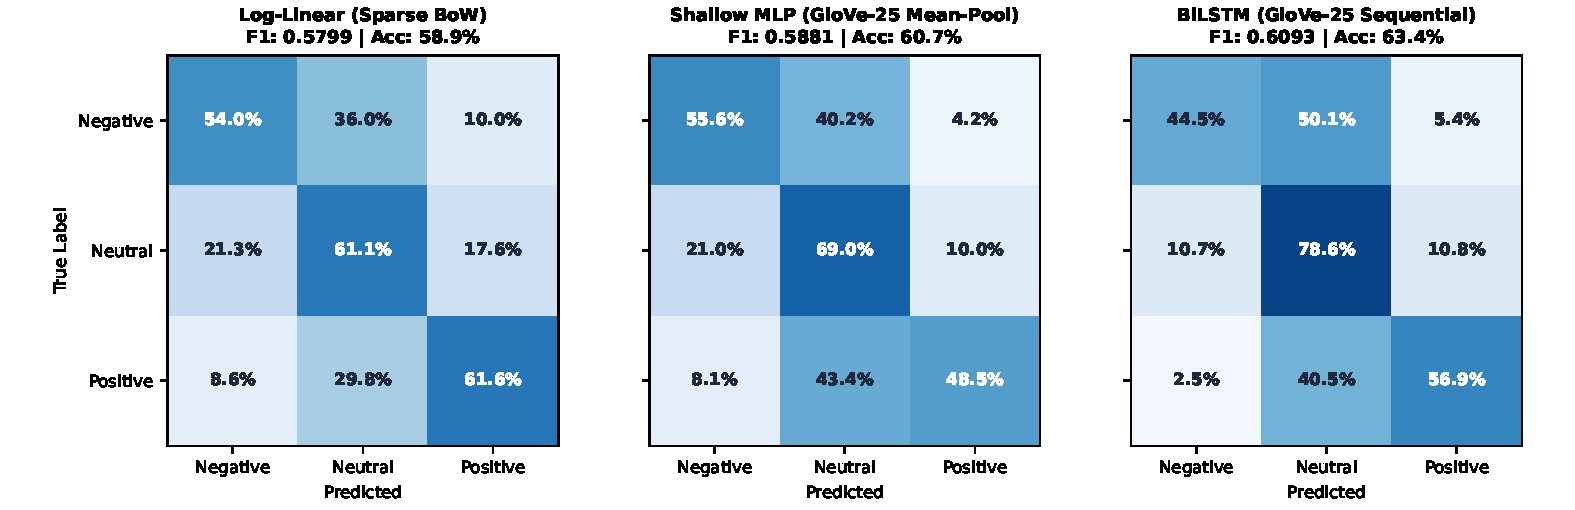
\includegraphics[width=\linewidth, height=0.68\textheight, keepaspectratio]{figures/minimal_confusion_matrices.pdf}
    \vspace{2pt}
    \begin{block}{Why Sequential Embeddings Win on Test}
        \scriptsize Reading GloVe embeddings sequentially resolves negation scope and syntactic assertions, unlocking $+2.12\%$ F1 and $+2.67\%$ accuracy over mean-pooled MLP!
    \end{block}
\end{column}
\end{columns}
\end{frame}

\end{document}
